\setcounter{secnumdepth}{0}
\section*{Dodatek F: Rozwiązania zadań}
\addcontentsline{toc}{section}{\protect\numberline{}Dodatek F: Rozwiązania zadań}

\subsection*{Rozwiązania wejściówki}
\begin{enumerate}
    \item Podaj definicję dodawania i mnożenia w $\mathbb{F}_2$ bądź wypisz wynik tych
    działań dla wszystkich możliwych kombinacji elementów.
    \begin{itemize}
        \item Odpowiedź: dodawanie to XOR a mnożenie to AND. Pozostałe możliwe odpowiedzi to Tablica~\ref{truth_table:title} bądź~(\ref{modulo_addition})
        oraz~(\ref{modulo_multiplication})
    \end{itemize}
    \item Czym się różni słowo kodowe wygenerowane kodem systematycznym i niesystematycznym
    \begin{itemize}
        \item Odpowiedź: słowo kodowe w kodowaniu systematycznym w przeciwieństwie do niesystematycznego zawiera w sobie kodowaną wiadomość, sekcja~\ref{subsection:Kod systematyczny}
    \end{itemize}
    \item Ile błędnych symboli jest w stanie wykryć lub poprawić kod Reeda-Solomona?
    \begin{itemize}
        \item Odpowiedź: wykryć: $n-k$, poprawić: $\lfloor \frac{n-k}{2} \rfloor$, sekcja~\ref{subsection:wlasciwosci}
    \end{itemize}
    \item Podaj zaletę oraz wadę stosowania większej ilości poziomów w modulacjach PAM.
    \begin{itemize}
        \item Odpowiedź: \\
        Zaleta:
        \begin{itemize}
            \item większa przepustowość bez zwiększania szerokości pasma.
        \end{itemize}
        Wady:
        \begin{itemize}
            \item zmniejszony stosunek sygnału do szumu,
            \item większa podatność na zakłócenia,
            \item konieczność używania dokładniejszych urządzeń.
        \end{itemize}
    \end{itemize}
    \item Opisz krótko czym jest NRZ (Non-Return-to-Zero).
    \begin{itemize}
        \item Odpowiedź: rodzaj kodowania o dwóch poziomach - dla 0 sygnał ujemny, dla 1 sygnał dodatni.
    \end{itemize}
\end{enumerate}

\subsection*{Rozwiązania ćwiczeń}
\begin{enumerate}
    \item Zakładka: Reed-Solomon, ustawienia programu: kod systematyczny BCH, $n=15$, $GF=2^4$.
    Dla $k \in \{ 2, 6, 10, 13 \}$ sprawdź wartość słowa kodowego dla k-symbolowej wiadomości zawierającej same zera. Dlaczego otrzymałeś takie słowa kodowe? \\ \\
    Odpowiedź: Otrzymaliśmy same zera ponieważ według wzoru z sekcji~\ref{subsubsection:systematic-bch} dla $p_m(x) = 0$ zawsze dostaniemy zera
    \begin{align*}
        c_r(x) &= 0 \cdot x^t \mod g(x) \\
        c_r(x) &= 0 \mod g(x) \\
        c_r(x) &= 0 \\
        c(x) &= 0 \cdot x^t - 0 \\
        c(x) &= 0
    \end{align*}

    Odpowiedź 2: Kod BCH jest kodem systematycznym dlatego pierwsze $k$ symboli
    także będzie miało zera. Aby obliczyć pozostałe $n-k$ symboli musimy mnożyć
    i dodawać przez 0 w związku z czym otrzymamy same zera.

    \begin{figure}[H]
        \centering
        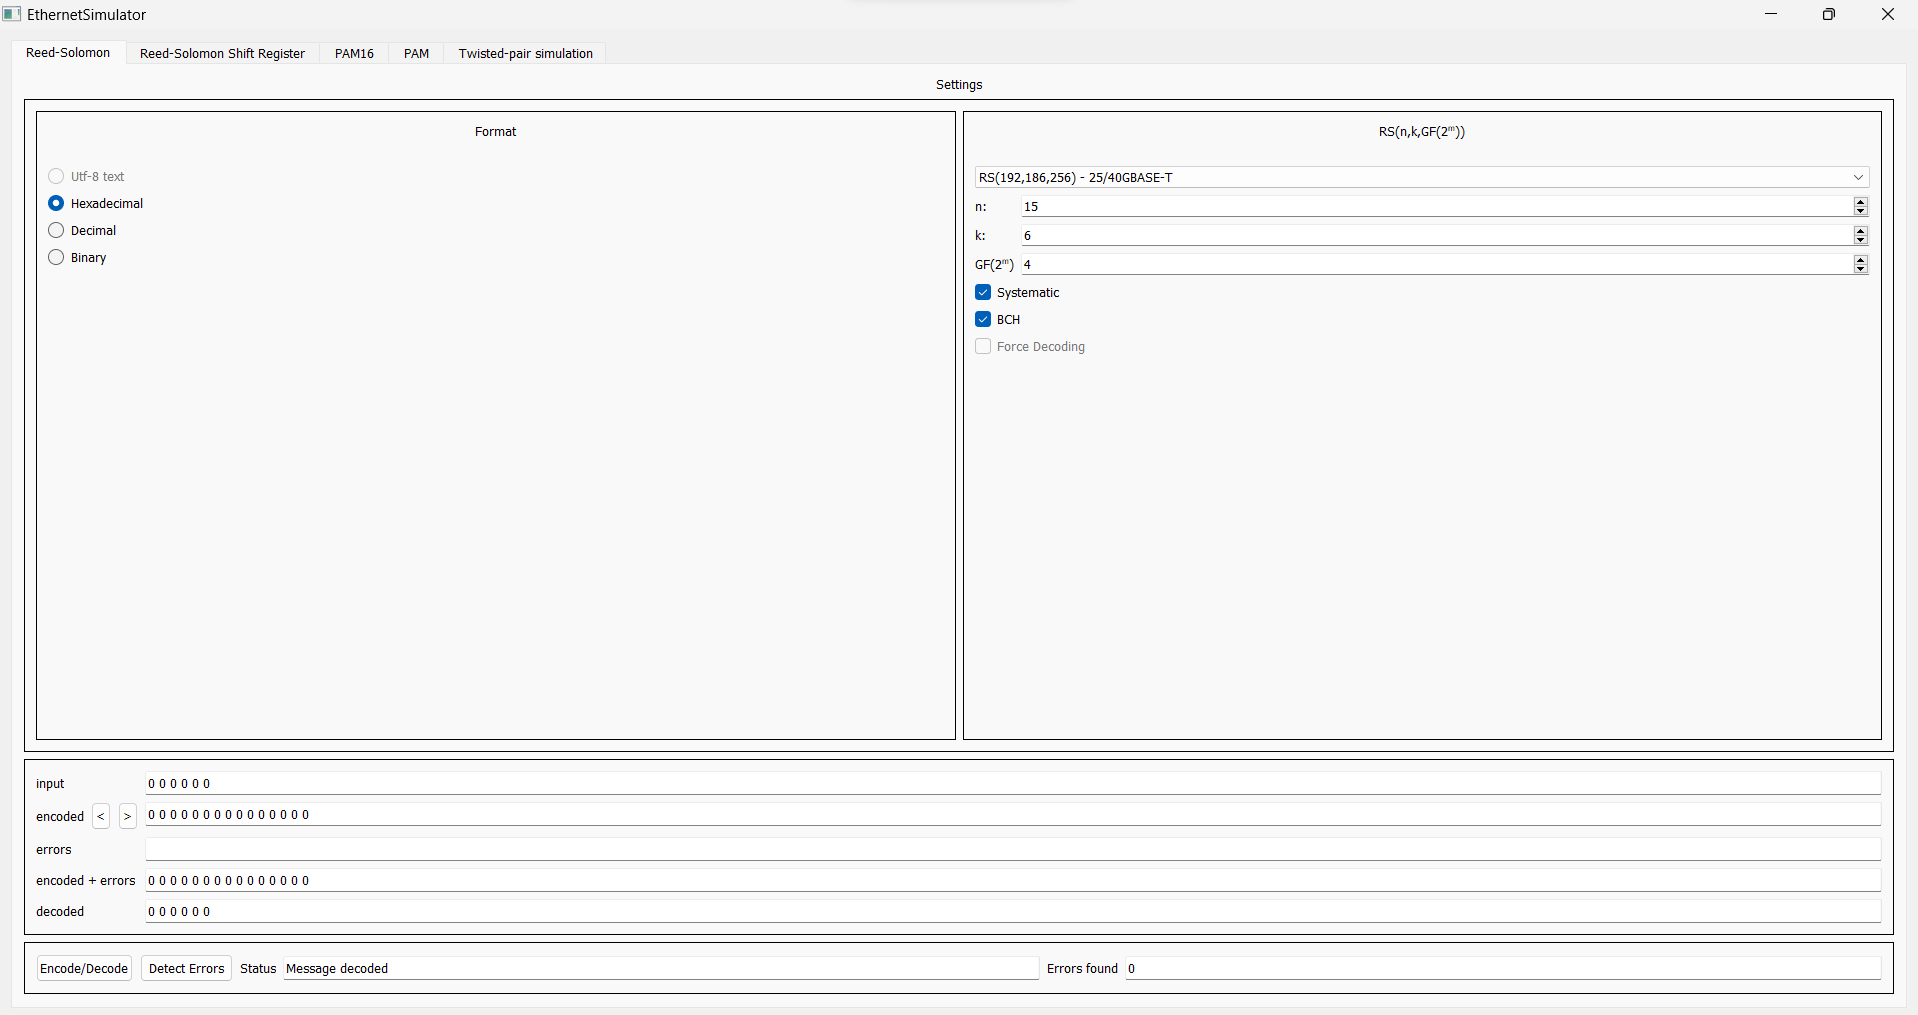
\includegraphics[width=\textwidth]{images/rozwiazania_1.png}
        \caption{Widok narzędzia Reed-Solomon podczas wykonywania zadania 1.}
        \label{fig:rozwiazania_1}
    \end{figure}
    
    \item Zakładka: Reed-Solomon, ustawienia programu: $n = 7$, $k = 3$, $GF = 2^3$,
    kod systematyczny BCH, tryb dziesiętny, wiadomość wejściowa `1 2 3'.
    Sprawdź dla błędów `3', `3 2', `3 2 1' oraz `3 2 1 4' czy dekoder jest w stanie
    wykryć błędy oraz czy jest w stanie je poprawić a jeżeli tak to czy poprawnie.
    Czy wiesz dlaczego pojawiły się rozbieżności między błędami poprawionymi a wykrytymi? \\ \\
    Odpowiedź: Według właściwości kodu Reeda-Solomona opisanych w sekcji~\ref{subsection:wlasciwosci} jest on w stanie poprawić $\lfloor \frac{n-k}{2} \rfloor$ błędnych symboli i wykryć $n-k$ błędnych symboli.
    W tym zadaniu wszystkie błędy były wykryte i jedynie $\lfloor \frac{n-k}{2} \rfloor$ czyli 2 błędy były poprawnie skorygowane.
    Odpowiedź 2: Ponieważ kod Reeda-Solomona jest w stanie wykryć 2 razy więcej
    błędów niż poprawić.
    \begin{table}[H]
        \renewcommand{\arraystretch}{1.8}
        \centering
        \begin{tabular}{|c|c|c|>{\centering\arraybackslash}p{5cm}|}
            \hline
            \textbf{Błąd} & \textbf{Wykrywa [TAK/NIE]} & \textbf{Poprawia [Ile]} & \textbf{Poprawia poprawnie [TAK/NIE]} \\
            \hline
            3 & TAK & 1 & TAK \\
            \hline
            3 2 & TAK & 2 & TAK \\
            \hline
            3 2 1 & TAK & 2 & NIE \\
            \hline
            3 2 1 4 & TAK & 2 & NIE \\
            \hline
        \end{tabular}
    \end{table}

    \begin{figure}[H]
        \centering
        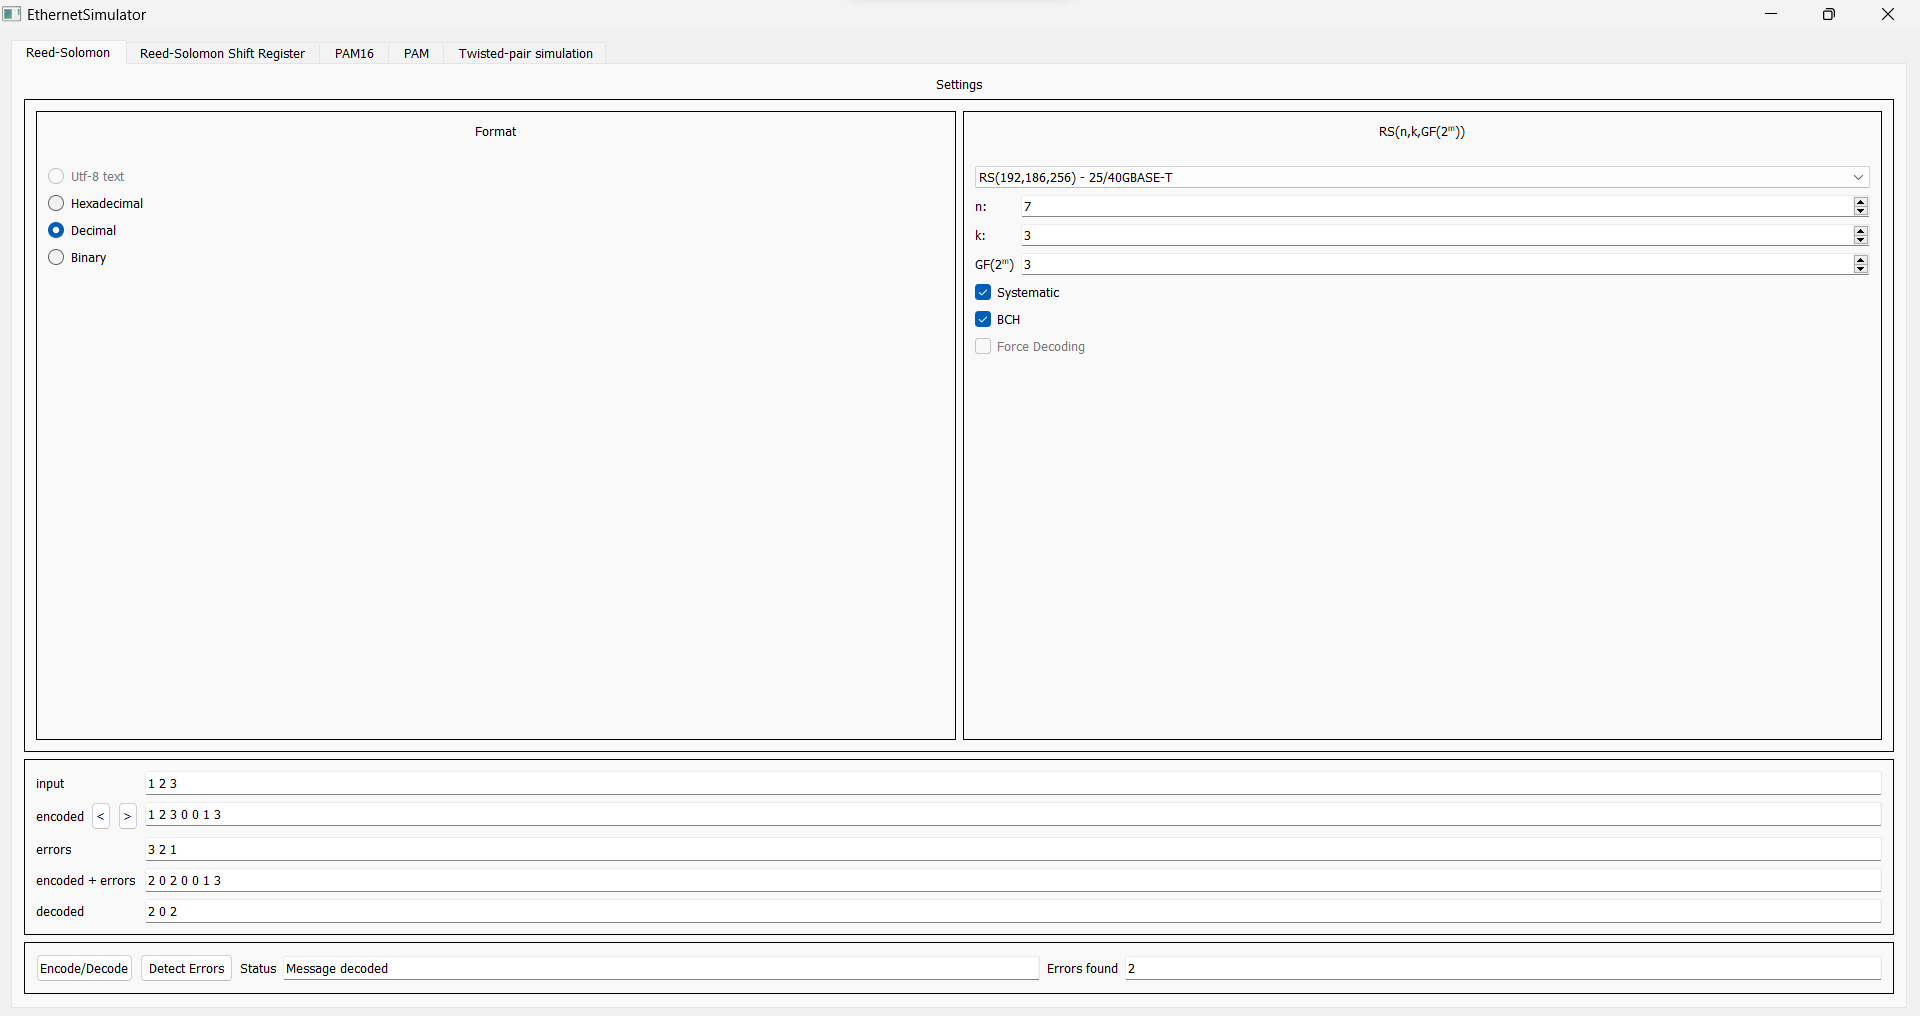
\includegraphics[width=\textwidth]{images/rozwiazania_2.png}
        \caption{Widok narzędzia Reed-Solomon podczas wykonywania zadania 2.}
        \label{fig:rozwiazania_2}
    \end{figure}
    
    \item Zakładka: Reed-Solomon Shift Register, ustawienia programu:
    $n = 3$, $k = 2$, $GF = 2^2$. Oblicz wielomian prymitywny i generator naciskając
    przycisk `Calculate primitive poly/element'.
    Zakoduj wiadomość: `2 1' w symulatorze po czym zakoduj wiadomość
    używając wzoru z sekcji `Systematyczny kod BCH'. Porównaj wyniki.
    \\ \\
    Odpowiedź: Zakodowana wiadomość to: `2 1 3'. Dla $p_m(x) = 2x + 1$ oraz $g(x) = x + 1$ słowo kodowe
    obliczone wzorem i przez symulator są takie same.
    \begin{equation*}
        \begin{aligned}[t]
            s_r(x) &= (2x+1) \cdot x \mod x + 1 \\
            s_r(x) &= 2x^2 + x \mod x + 1 \\
            s_r(x) &= 3 \\
            s(x) &= (2x+1) \cdot x - s_r(x) \\
            s(x) &= 2x^2 + x + 3 \\
            s(x) &= (2,1,3)
        \end{aligned}
    \end{equation*}

    

    \begin{figure}[H]
        \centering
        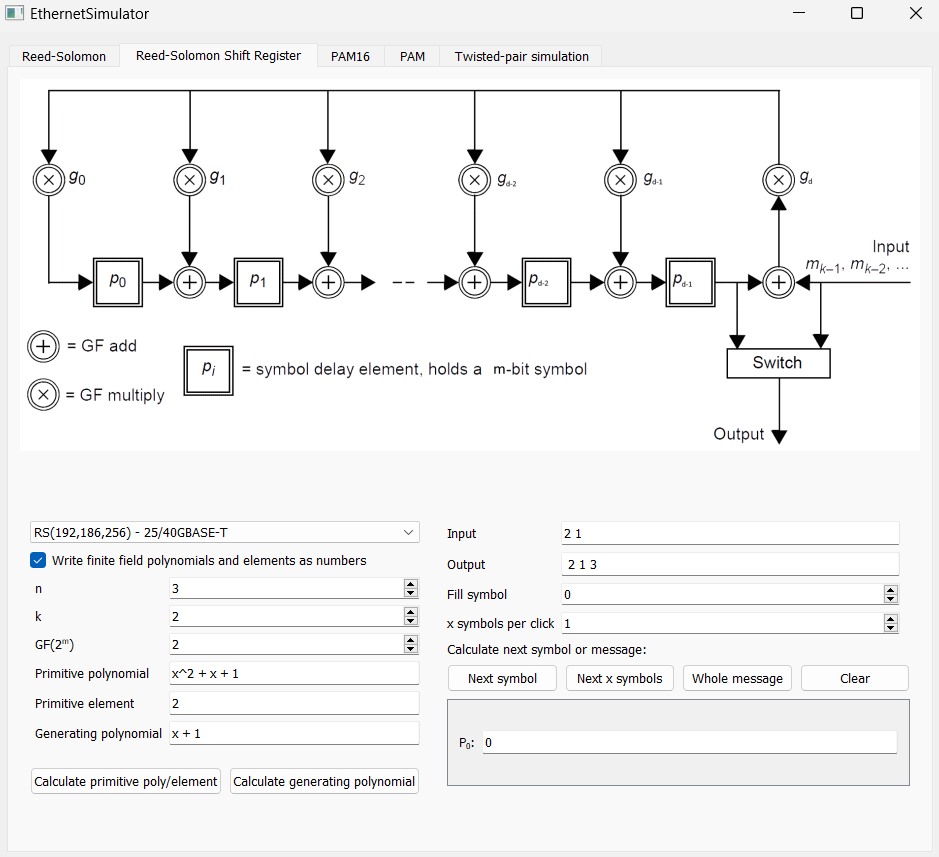
\includegraphics[width=\textwidth]{images/rozwiazania_3.png}
        \caption{Widok narzędzia Reed-Solomon Shift Register podczas wykonywania zadania 3.}
        \label{fig:rozwiazania_3}
    \end{figure}
    
    \item Zakładka: Reed-Solomon, ustawienia programu: $n = 15$, $k=7$, $GF = 2^4$,
    kod systematyczny BCH.
    Zakoduj dowolną niezerową $k$-symbolową wiadomość. Sprawdź czy przesunięcia słowa kodowego
    (z użyciem strzałek przy słowie `encoded') także będą słowem kodowym. \\ \\
    Odpowiedź: Dla wiadomości `1 2 3 4 5 6 7' wszystkie przesunięcia były poprawnie i bezbłędnie dekodowane.
    

    \begin{figure}[H]
        \centering
        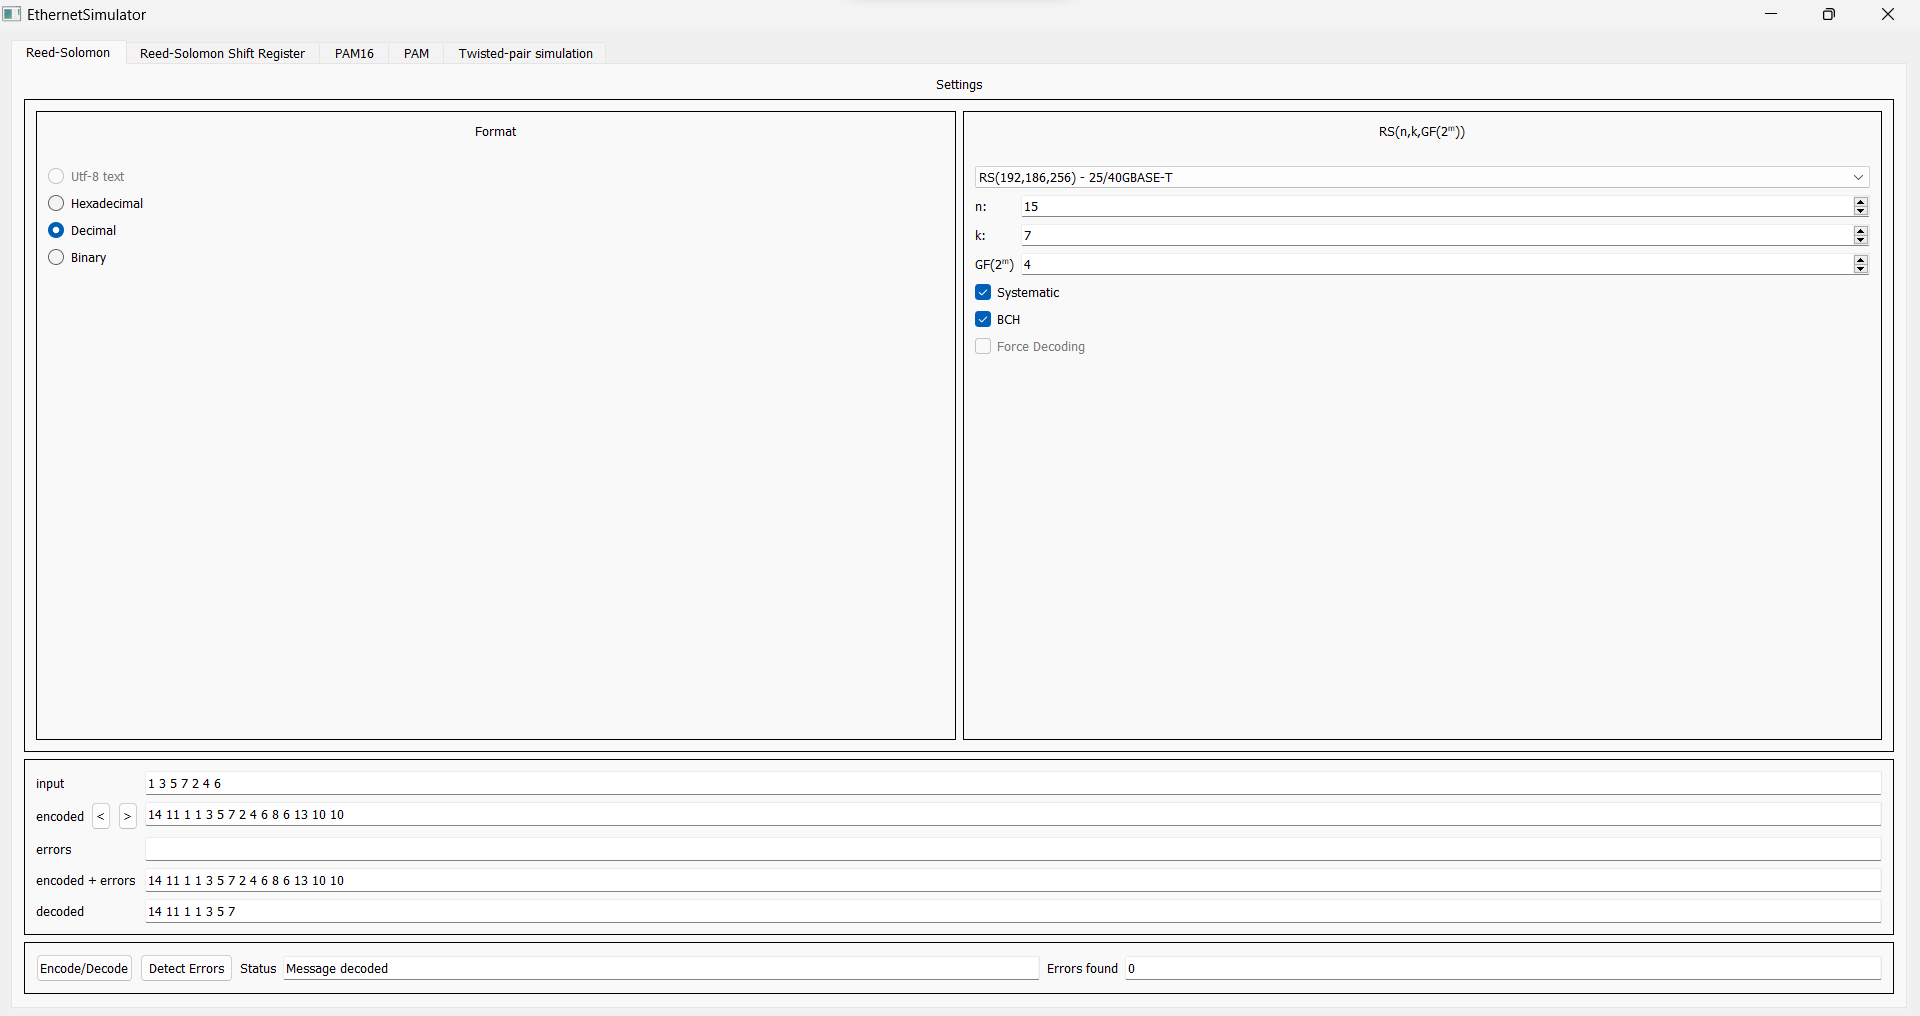
\includegraphics[width=\textwidth]{images/rozwiazania_4.png}
        \caption{Widok narzędzia Reed-Solomon podczas wykonywania zadania 4.}
        \label{fig:rozwiazania_4}
    \end{figure}
    
    \item Zakładka: PAM, Zamień numer swojego indeksu na postać szesnastkową i wykorzystaj go jako liczbę do przesłania. Przeprowadź symulację. Zanotuj w sprawozdaniu
    przybliżony czas transmisji oraz liczbę poziomów natężenia. Opisz wnioski, które nasuwają Ci się po wykonanym ćwiczeniu. \\ \\
    Odpowiedź:
    \begin{itemize}
        \item NRZ: 62ns, dwa poziomy
        \item PAM4: 33ns, cztery poziomy
        \item PAM16: 17ns, cztery poziomy (przesyłany numer indeksu jest na tyle mały, że nie wszystkie poziomy zostaną wykorzystane)
    \end{itemize}
    Stosowanie modulacji PAM wyższych poziomów pozwala na lepsze upakowanie danych, ale różnica pomiędzy wysyłanymi symbolami maleje.
    

    \begin{figure}[H]
        \centering
        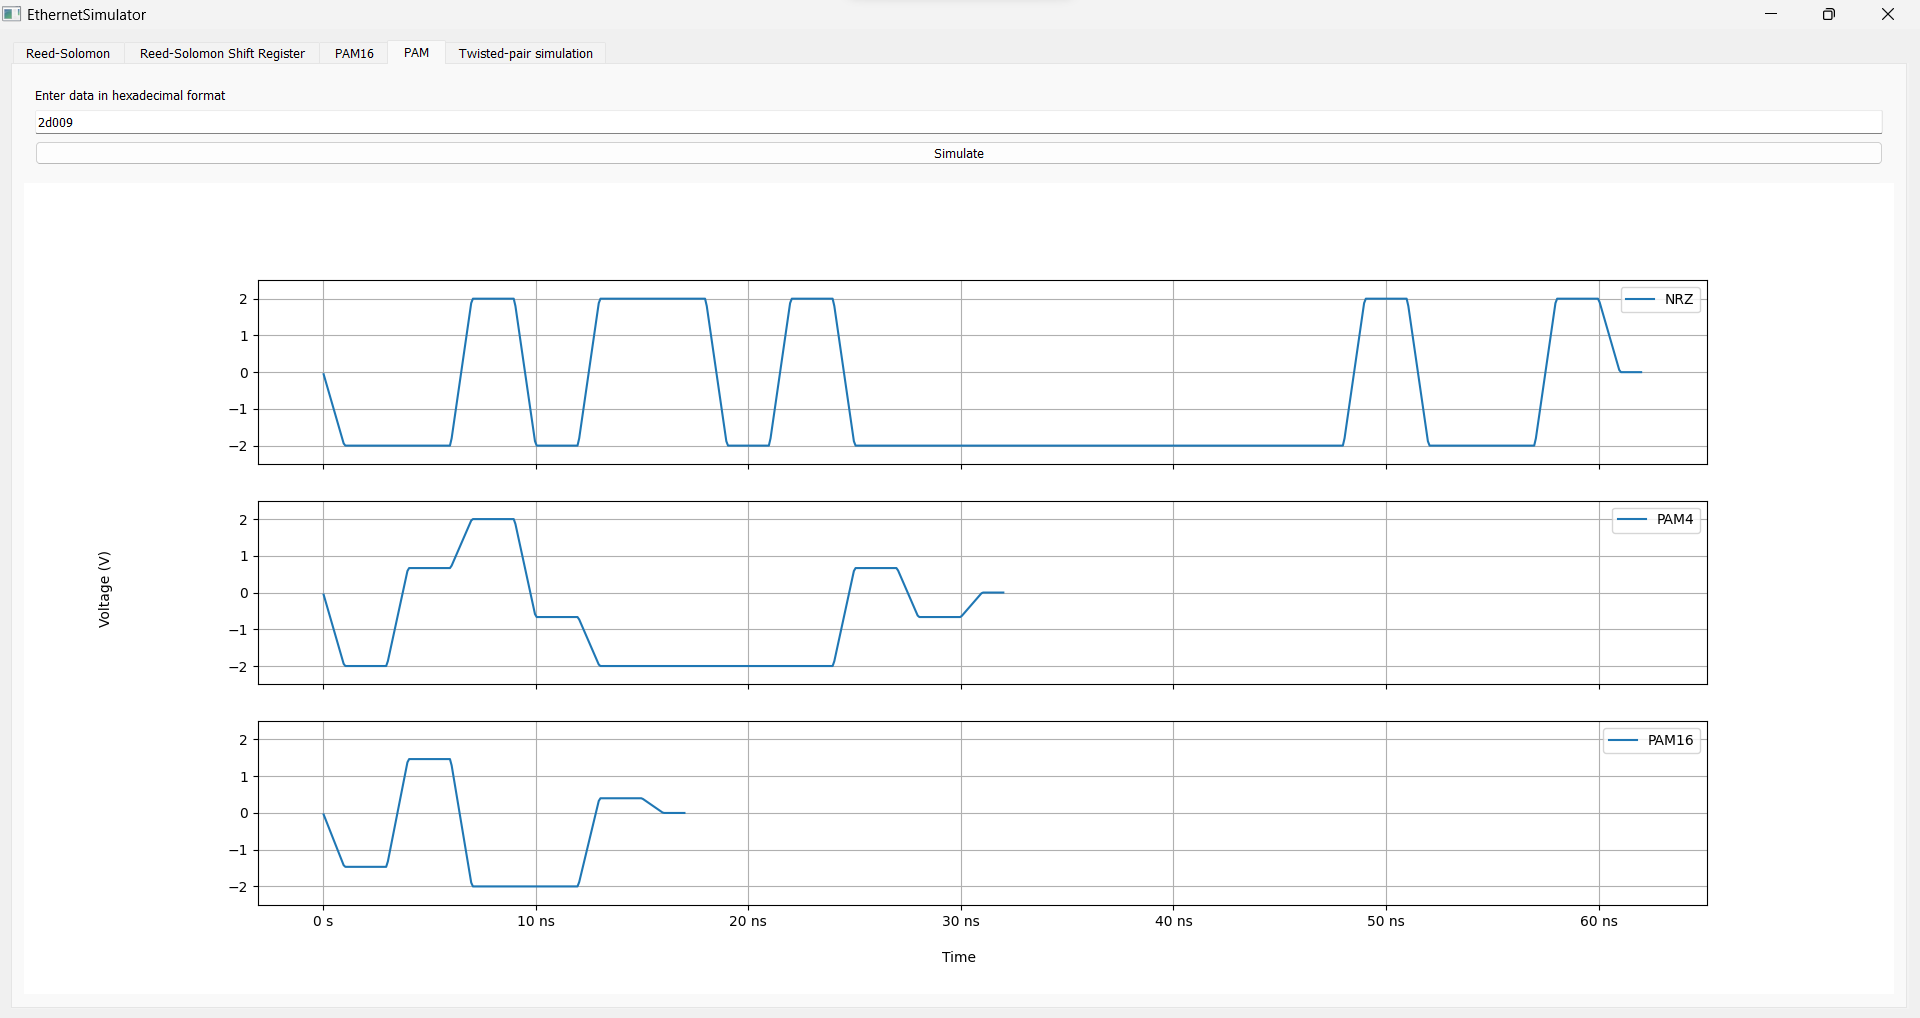
\includegraphics[width=\textwidth]{images/rozwiazania_5.png}
        \caption{Widok narzędzia PAM podczas wykonywania zadania 5.}
        \label{fig:rozwiazania_5}
    \end{figure}
    
    \item Zakładka: PAM, Prześlij ciąg składający się z samych jedynek (fffffff \dots) lub zer (000000 \dots). Popatrz na wynik symulacji. Jak nazywa się zaobserwowane zjawisko? Czy znasz sposoby,
    które zapobiegają jego wystąpieniu? Zanotuj w sprawozdaniu. \\ \\
    Odpowiedź: Na symulacji widać stałą składową. Można jej zapobiegać używając np. kodowania liniowego 64b/66b albo skramblera.
    
    

    \begin{figure}[H]
        \centering
        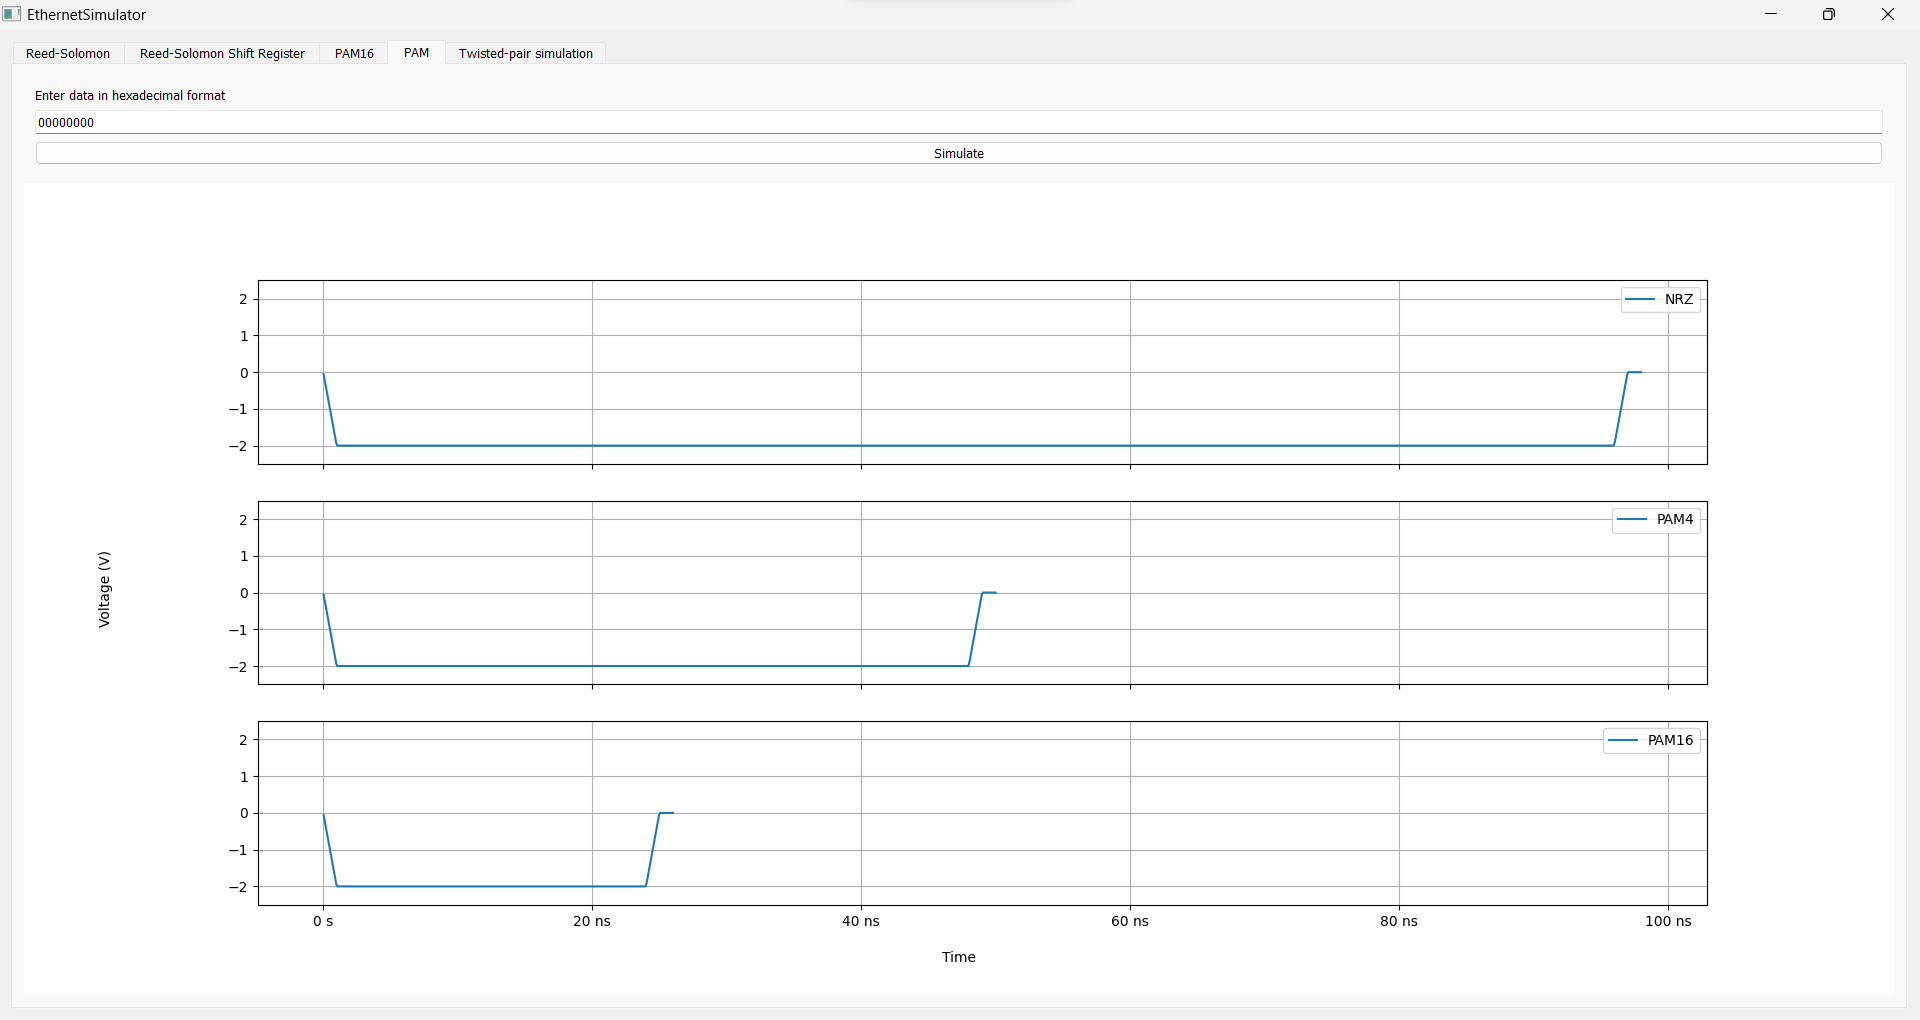
\includegraphics[width=\textwidth]{images/rozwiazania_6.png}
        \caption{Widok narzędzia PAM podczas wykonywania zadania 6.}
        \label{fig:rozwiazania_6}
    \end{figure}
    
    \item Zakładka: PAM16, Zastosowanie DSQ128 nie eliminuje możliwości wystąpienia stałej składowej. Znajdź ciąg, który
    temu dowodzi i zanotuj go w sprawozdaniu. \\ \\
    Odpowiedź: Na przykład: 0x000000 \dots, 0x111111 \dots (0b000100010001 \dots),\\0x22222 \dots (0b001000100010 \dots),
    0x444444 \dots (0b010001000100 \dots).

    

    \begin{figure}[H]
        \centering
        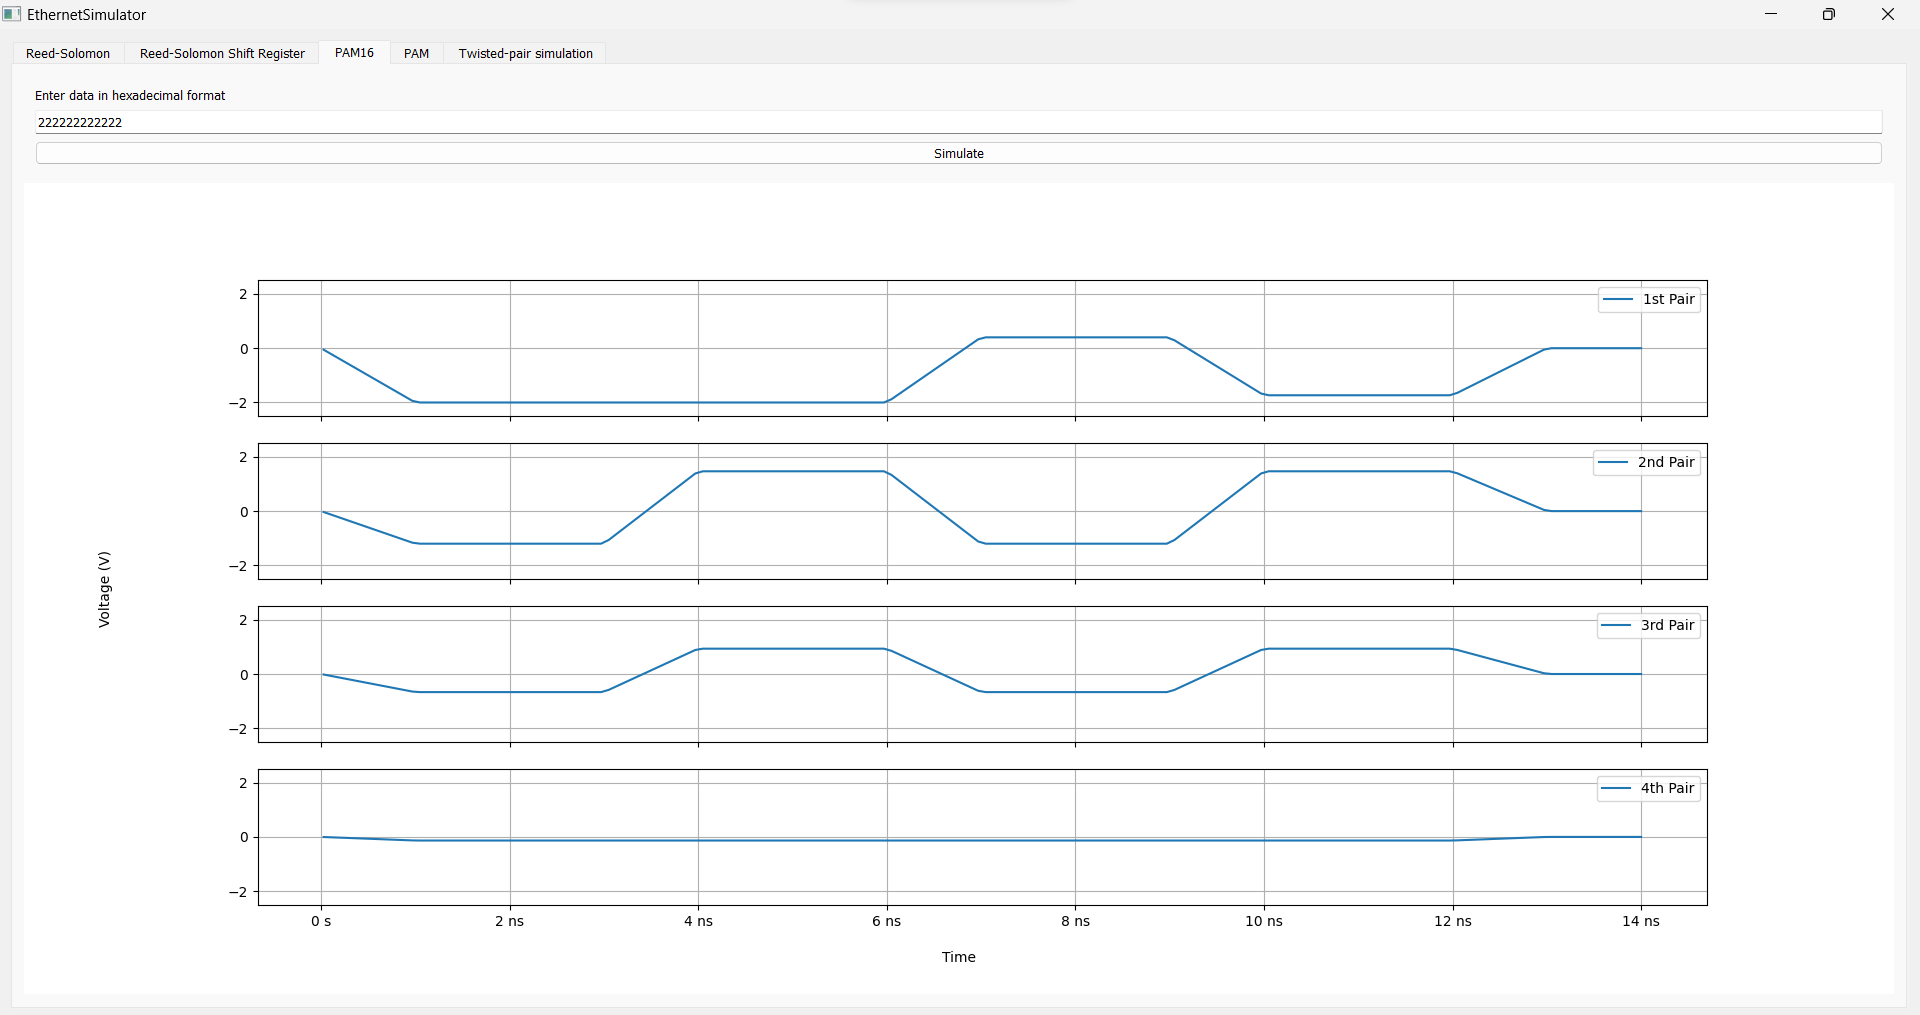
\includegraphics[width=\textwidth]{images/rozwiazania_7.png}
        \caption{Widok narzędzia PAM podczas wykonywania zadania 7.}
        \label{fig:rozwiazania_7}
    \end{figure}
    
    \end{enumerate}

\subsection*{Wnioski}

W naszej ocenie przygotowane w ramach niniejszej pracy zadania laboratoryjne powinny w dobry sposób przybliżyć studentom podstawy
teoretyczne oraz aspekty praktyczne poruszanych w nich zagadnień. Zadania są krótkie i stosunkowo łatwe do rozwiązania, dzięki czemu
student nie jest poddany presji czasu. Zaprojektowany symulator wizualizuje omawiane rozwiązania warstwy fizycznej Ethernet, co byłoby
trudne i wymagałoby wysokiej jakości sprzętu, jeżeli realizacja przebiegałaby na rzeczywistym sprzęcie.
